% !TeX program = lualatex
% !TeX encoding = utf8
% !TeX spellcheck = uk_UA

\documentclass[]{beamer}
\usetheme{PlasmaPhysics}
\usepackage{PlasmaPhysics}
\usepackage{subcaption}
\usepackage{mathtools}
\setlength{\abovedisplayskip}{3pt}
\setlength{\belowdisplayskip}{3pt}
\usetikzlibrary{decorations.pathreplacing}
\newtcolorbox{mysidebyside}[1][]{
    notitle, sidebyside, blanker,
    sidebyside align=center seam,
    halign=center,
    lefthand width=.5\textwidth,
    #1
}



\graphicspath{{pictures/}}
\title[Лекції з фізики плазми]{\bfseries\huge Рух заряджений частинок в плазмі 2}
\subtitle{\bfseries Лекції з фізики плазми}
\author{Пономаренко С. М.}
\date{}
% https://www.youtube.com/watch?v=zv9Y7YmHyBk
\def\stext#1{\text{
        \makebox[0pt]{
            \tikz[baseline] {\node[text width=50pt, align=center, execute at begin node=\setlength{\baselineskip}{-0.5ex}, blue] {#1};}
        }
}}


\begin{document}




%===============================================================================
\usebackgroundtemplate{
	\tikz\node[opacity=0.1]{\includegraphics[width=\paperwidth,height=\paperheight]{background}};%
}


\begin{frame}
	\thispagestyle{empty}
	\titlepage
\end{frame}


% ============================== Слайд ## ===================================
\begin{frame}{Магнітний момент}{}
	\begin{block}{Магнітний момент}
		\begin{equation*}
			p_m = \frac1c IS = \frac1c \frac{Ze \Omega}{2\pi}\pi\rho^2 = \frac1c \frac{Zev^2_\perp}{2\Omega} = \frac{mv^2_\perp}{2B}.
		\end{equation*}
	\end{block}
	\begin{center}
		\tdplotsetmaincoords{60}{0}
\begin{tikzpicture}[>=latex, tdplot_main_coords]
	\tdplotsetrotatedcoords{0}{20}{0}
    % -------------- ion -----------------
	\begin{scope}[tdplot_rotated_coords]
		\coordinate (O) at (0,0,0);
		\coordinate (z) at (0,0,1.5);
		\coordinate (x) at (1,00);
		\coordinate (y) at (0,1,0);
		\coordinate (-z) at (0,0,-1.5);
       	\coordinate (p) at (0,0,-2);

		%    \draw[->] (O) -- (y) node[anchor=south] {$y$};
		%    \draw[->] (O) -- (x) node[anchor=south] {$x$};

		\draw[->, gray, thick] (O) -- (z) node[anchor=south] {$\vec{B}$};
        \draw[->, orange, thin] (O) -- (p) node[anchor=east] {$\vec{p}_m$};
		\draw[->, blue, thick] (O) -- (-z) node[anchor=west] {$\vec\Omega$};
		\draw[canvas is xy plane at z=0,
			draw=blue,
            thick,
			decoration={markings,
					mark=at position 0.75 with {\arrow[rotate=180, xshift=2pt]{latex}},
				},
			postaction=decorate,
		] (0,0) ++(90 :1) arc [start angle=90, delta angle=335, radius=1];

		\begin{scope}[canvas is xy plane at z=0]
            \node[circle, fill=blue, inner sep=1pt] at (0,0) {};
			\node[transform shape=false, ball color=blue, circle, inner sep=0, text=white] at (45:1) {$+$};
		\end{scope}

        % -------------- electron -----------------
		\begin{scope}[xshift=3cm]
			\coordinate (O) at (0,0,0);
			\coordinate (z) at (0,0,1.5);
			\coordinate (x) at (1,00);
			\coordinate (y) at (0,1,0);
			\coordinate (w) at (0,0,1.25);
           	\coordinate (p) at (0,0,-2);

			%    \draw[->] (O) -- (y) node[anchor=south] {$y$};
			%    \draw[->] (O) -- (x) node[anchor=south] {$x$};

			\draw[->, gray, thick] (O) -- (z) node[anchor=south] {$\vec{B}$};
			\draw[->, red, thick] (O) -- (w) node[anchor=north west] {$\vec\Omega$};
            \draw[->, orange, thin] (O) -- (p) node[anchor=east] {$\vec{p}_m$};
			\draw[canvas is xy plane at z=0,
				draw=red,
                thick,
				decoration={markings,
						mark=at position 0.2 with {\arrow[xshift=2pt]{latex}},
					},
				postaction=decorate,
			] (0,0) ++(90 :1) arc [start angle=90, delta angle=335, radius=1];

			\begin{scope}[canvas is xy plane at z=0]
                \node[circle, fill=blue, inner sep=1pt] at (0,0) {};
				\node[transform shape=false, ball color=red, circle, inner sep=1pt, text=white] at (105:1) {\tikz\draw[]  (0,0) -- ++(0.1,0);};
			\end{scope}
		\end{scope}
	\end{scope}
\end{tikzpicture}
	\end{center}

	\begin{block}{Магнітний момент ларморового кільця}
		\begin{equation*}
			\vec{p}_m = -\frac{mv^2_\perp}{2B^2}\vec{B}, \quad p_m = \frac{mv^2_\perp}{2B}
		\end{equation*}
	\end{block}
\end{frame}
% ===========================================================================


% ============================== Слайд ## ===================================
\begin{frame}{Діамагнетизм плазми}{}
	\begin{tblr}{Q[l, m, 0.6\linewidth]X[c, m, mode=dmath]}
		Намагніченість плазми:
		 &
		\vec{M} = n\vec{p}_m =  -\frac{nmv^2_\perp}{2B^2}\vec{B}
		\\
		Зв'язок намагніченості з напруженістю магнітного поля:
		 &
		\vec{M} = \chi \vec{H}
		\\
		Магнітна сприйнятливість плазми:
		 &
		\chi = -\frac{nmv^2_\perp}{2B^2} < 0
	\end{tblr}


	\begin{block}{Ідея утримання плазми (І. Тамм, Д. Сахаров, 1950)}\justifying
		Для плазми $\chi < 0$, це означає, що плазма має \alert{діамагнітні властивості}, тобто, вона має \alert{виштовхуватися з області сильного поля}. На цій властивості ґрунтується ідея магнітного утримання плазми: необхідно створити магнітні <<корки>> або <<дзеркала>>, від яких плазма відштовхуватиметься, внаслідок чого вона утримуватиметься в обмеженій ділянці простору, не торкаючись стінок камери.
	\end{block}

\end{frame}
% ===========================================================================

% ============================== Слайд ## ===================================
\begin{frame}{Рух частинки в неоднорідному полі $\nabla B \parallel \vec{B}$}
\framesubtitle<1>{Рівняння руху}
\framesubtitle<2>{Закон збереження енергії. Інваріантність магнітного моменту ларморового кільця}
            На частинку діамагнетика діє сила:
            \begin{equation*}
                \vec{F} = -\vec{p}_m\nabla_\parallel B.
            \end{equation*}
   		\emph{}\begin{figure}[h!]
%---------------------------------------------------------
\begin{subfigure}[t]{0.45\linewidth}\centering
		\begin{tikzpicture}[>=latex']
			\draw[red, ->, domain=1:4] plot({\x}, {1/\x});
			\draw[red, ->] (1, 0) -- (4,0);
			\draw[red, ->, domain=1:4] plot({\x}, {-1/\x});
            \foreach \xc in {2} {

            \draw[blue!55, ultra thick] (\xc, 0) [partial ellipse=-90:90:{0.5*1/\xc} and {1/\xc}];

       		\draw[->, green!70!black, thick] (\xc, 0) -- ++(1.5/\xc, 0) node[inner sep=1pt, anchor=north west, font=\tiny, text=black] {$\vec{v}_\parallel$};
            \draw[->, orange, thick] (\xc, 0) -- ++(-0.75, 0) node[inner sep=1pt, anchor=north east, font=\tiny, text=black] {$\vec{F}$};

       		\draw[blue!60, ultra thick,
       			decoration={markings,
       					mark=at position 0.7 with {\arrow[xshift=2pt,scale=0.7]{>}},
       					mark=at position 0.3 with {\node[circle, ball color=blue!60, text=white, inner sep=0, font=\tiny] {$+$};},
       				},
       			postaction={decorate}] (\xc, 0) [partial ellipse=-45:-315:{0.5*1/\xc} and {1/\xc}];
            }
		\end{tikzpicture}
\end{subfigure}
%---------------------------------------------------------
\begin{subfigure}[t]{0.45\linewidth}\centering
		\begin{tikzpicture}[>=latex']
			\draw[red, ->, domain=1:4] plot({\x}, {1/\x});
			\draw[red, ->] (1, 0) -- (4,0);
			\draw[red, ->, domain=1:4] plot({\x}, {-1/\x});

			\foreach \xc in {1.5, 3} {

            \draw[blue!55, ultra thick] (\xc, 0) [partial ellipse=-90:90:{0.5*1/\xc} and {1/\xc}];


					\draw[->, green!70!black, thick] (\xc, 0) -- ++(1.5/\xc, 0) node[inner sep=1pt, anchor=north west, font=\tiny, text=black] {$\vec{v}_\parallel$};
                    \draw[blue!60, ultra thick,
                           			decoration={markings,
                           					mark=at position 0.7 with {\arrow[xshift=2pt,scale=0.7]{>}},
                           					mark=at position 0.3 with {\node[circle, ball color=blue, text=white, inner sep=0, font=\tiny] {$+$};},
                           				},
                           			postaction={decorate}] (\xc, 0) [partial ellipse=-45:-315:{0.5*1/\xc} and {1/\xc}];

				}
		\end{tikzpicture}
\end{subfigure}
%---------------------------------------------------------
\end{figure}

\begin{overprint}
\onslide<1>
        Рівняння руху вздовж осі $z$:
        \begin{equation*}
            m\frac{dv_\parallel}{dt} = -p_m\frac{\partial B}{\partial z}.
        \end{equation*}
        \begin{equation*}
            m{\color{red}v_\parallel}\frac{dv_\parallel}{dt} = -p_m\frac{d B}{d z}{\color{red}\frac{dz}{dt}}  \Rightarrow \frac{d}{dt}\left(\frac{mv^2_\parallel}{2} \right) + p_m\frac{dB}{dt} = 0.
        \end{equation*}
\onslide<2>
Закон збереження енергії:
\begin{equation*}
 \frac{d}{dt}\left(\frac{mv^2_\parallel}{2} + \frac{mv^2_\perp}{2} \right) = \frac{d}{dt}\left(\frac{mv^2_\parallel}{2} + p_mB \right) = 0.
\end{equation*}
\begin{equation*}
    \frac{d}{dt} \left( p_mB\right) = p_m\frac{dB}{dt} = 0 \Rightarrow \frac{dp_m}{dt} = 0 \Rightarrow \tcbhighmath{p_m = \const.}
\end{equation*}
\end{overprint}
\end{frame}
% ===========================================================================





% ============================== Слайд ## ===================================
\begin{frame}{Магнітне дзеркало}{}
\begin{onlyenv}<1-3>
    \begin{block}{}
         Неоднорідне магнітне поле, що створене парою котушок, утворює два магнітних дзеркала, між якими можна замкнути плазму.
    \end{block}
       \begin{center}
       \begin{tikzpicture}[>=latex',
    declare function={
    w=3;
    v=0.5;
    a=0.025;
    R(\t)=1/sqrt(4+5*\t);
    x(\t)=v*\t - a*\t^2;
    y(\t)=R(\t)*cos(w*\t r);
    },
]


	\foreach \i in {-1, 1} {
			\draw[thick, red!20, ultra thick] (\i*2.5,0) [partial ellipse=-40:40:0.15cm and 0.5cm];
		}
	\foreach \f in {-1,-0.75,...,1}{
			\draw[
				blue!40,
				yscale=\f,
				postaction={decorate, decoration={markings, mark=at position 0.99 with {\arrow[scale=0.75]{latex}}}}
			] (-3, 0.5) to[out=-45, in=-135] (-2, 0.5) to[out=45, in=135] (2, 0.5) to[out=-45, in =-135] (3,0.5);
		}

	\foreach \i in {-1, 1} {
			\draw[thick, red!50, ultra thick,
				postaction={decorate, decoration={markings, mark=at position 0.5 with {\arrow[scale=0.5]{latex}}}}
			] (\i*2.5,0) [partial ellipse=40:320:0.15cm and 0.5cm];
		}


    \draw[->] (0,0) -- ++(0, 0.5) node[left, font=\scriptsize] {$\vec{v}_\perp$};
    \draw[->] (0,0) -- ++(1, 0) node[right, font=\scriptsize] {$\vec{v}_\parallel$};;
    \draw[->] (0,0) -- ++(1, 0.5) node[above, font=\scriptsize] {$\vec{v}$};;
    \draw[densely dashed] (0,0.5) -- ++(1,0) -- ++(0,-0.5);
    \draw[] (0,0) ++(0.5, 0) arc[start angle=0, delta angle=atan(0.5), radius=0.5] node[pos=0, inner sep=1pt, anchor=north west, font=\scriptsize] {$\theta_{\min}$};

        \draw[red!80, domain=0:4.9*pi, variable=\t, samples=300, ->] plot ({x(\t)}, {y(\t)} );

\end{tikzpicture}
       \end{center}
\end{onlyenv}
     \begin{overprint}
     \onslide<1>%
     \begin{block}{}
         Така пастка недосконала. Зокрема, частинка з $v_\perp = 0$, яка не має магнітного моменту, взагалі не відчує жодної сили, що діє вздовж $B$.
     \end{block}
     \begin{alertblock}{}
         Який мінімальний кут $\theta_{\min}$ повинна мати частинка, щоб утриматись в середині пастки?
     \end{alertblock}
     \onslide<2>%
     Із законів збереження:
     \begin{equation*}
         \frac{mv^2_{\perp\min}}{2B_{\min}} = \frac{mv^2_{\perp\max}}{2B_{\max}}, \quad
         \frac{v^2_{\perp\min}}{\sin^2\theta_{\min}} = v^2_{\perp\max}. \Rightarrow \tcbhighmath{\frac{B_{\min}}{B_{\max}} = \sin^2\theta_{\min}.}
     \end{equation*}
     \onslide<3>%
     \begin{block}{Дзеркальне відношення $R_m$}
              \begin{equation*}
                  \frac{B_{\min}}{B_{\max}} = \sin^2\theta_{\min} = \frac1{R_m}.
              \end{equation*}
          Умова $\theta > \theta_{\min}$, виділяє в просторі швидкостей область утримання зарядженої частинки. Кут $\theta$ називається \alert{пітч-кутом орбіти в області слабкого поля}.
     \end{block}
     \end{overprint}
\end{frame}
% ===========================================================================




% ============================== Слайд ## ===================================
\begin{frame}{Конус втрат}{}
\begin{columns}
	\begin{column}{0.3\linewidth}
         \begin{center}
             \tdplotsetmaincoords{80}{100}

\begin{figure}[!h]
	\centering



	\begin{tikzpicture}[tdplot_main_coords, grid/.style={help lines,violet!40!white},scale=1, >=latex',
			declare function={
					r=3;
					th=30;
					ph=45;
					x(\r,\th,\ph)=\r*sin(\th)*cos(\ph);
					y(\r,\th,\ph)=\r*sin(\th)*sin(\ph);
					z(\r,\th)=\r*cos(\th);
				},
		]
		\coordinate (O) at (0,0,0);

		\tdplotsetrotatedcoords{ph}{0}{0}
		\draw[->] (O) -- (5,0,0) node[anchor=north east, inner sep=1pt] {$v_x$};
		\draw[->] (O) -- (0,2,0) node[right] {$v_y$};
		\draw[->] (O) -- (0,0,{z(r,th)}) node[above] {$v_\parallel$} coordinate (vpar);
		\draw[->] (O) -- ({x(r,th,ph)}, {y(r,th,ph)}, {z(r,th)}) node[above] {$\vec{v}$} coordinate (v);

		\draw[->] (O) -- ({x(r,th,ph)}, {y(r,th,ph)}, 0) node[below] {$\vec{v}_\perp$} coordinate (vperp);

		\draw[densely dashed] (vperp) -- (v) -- (vpar);

		\foreach \p in {0,0.02,...,1.5}
			{
				\draw[canvas is xy plane at z=\p, blue!20,opacity=0.5] circle[radius=\p*2/3];
				\draw[canvas is xy plane at z=-\p, blue!20,opacity=0.5] circle[radius=\p*2/3];
			}

		%  \tdplotgetpolarcoords{x(1.5,atan(2/3),0)}{0}{z(1.5,atan(2/3),0)}
		%      \draw[densely dashed] (O) -- ({x(1.5,atan(2/3),0)}, 0, {z(1.5,atan(2/3),0)});
		%    \tdplotsetthetaplanecoords{\tdplotresphi}
		%    \tdplotdrawarc[tdplot_rotated_coords]{(0,0,0)}{1}{0}%
		%    {\tdplotrestheta}{inner sep=1pt, anchor=south west}{$\theta$}

		\tdplotgetpolarcoords{x(r,th,ph)}{y(r,th,ph)}{z(r,th)}
		\tdplotsetthetaplanecoords{\tdplotresphi}
		\tdplotdrawarc[tdplot_rotated_coords]{(0,0,0)}{0.75}{0}%
		{\tdplotrestheta}{inner sep=2pt, anchor=south}{$\theta$}

	\end{tikzpicture}
\end{figure}
         \end{center}
	\end{column}
    \quad%
	\begin{column}{0.6\linewidth}
        \begin{block}{}\justifying
        \begin{equation*}
        \tcbhighmath{
           \frac1{R_m} = \frac{B_{\min}}{B_{\max}} = \sin^2\theta_{\min}.
           }
        \end{equation*}
            Умова $\theta > \theta_{\min}$, виділяє в просторі швидкостей область утримання зарядженої частинки. Кут $\theta$ називається \alert{пітч-кутом орбіти в області слабкого поля}.
        \end{block}
	\end{column}
\end{columns}
    \begin{block}{}\justifying\scriptsize
        Частинки, швидкості яких лежать усередині конуса, не утримуються магнітними пробками. Форма конуса втрат не залежить від $q$ і $m$ і за відсутності зіткнень пастка буде утримувати як іони, так і електрони. За наявності в системі зіткнень частинки можуть виходити з пастки.  Зазвичай електрони виходять із пастки швидше, ніж іони, оскільки частота зіткнень у них вища. Тому в плазмі в ділянці $B_{\max}$ має виникнути \alert{амбіполярне електричне поле}, яке вирівнює потоки частинок обох знаків, що залишають плазму, і забезпечує її квазінейтральність.
    \end{block}
\end{frame}
% ===========================================================================






% ============================== Слайд ## ===================================
\begin{frame}{Радіаційні пояси Землі}{}
       \begin{block}{}\justifying
           Радіаційні пояси складаються з частинок, що застрягли в магнітному полі Землі --- електронів та іонів.
       \end{block}
       %=========================================================
       \begin{figure}[h!]\centering
       %---------------------------------------------------------
       \begin{subfigure}[t]{0.45\linewidth}\centering
           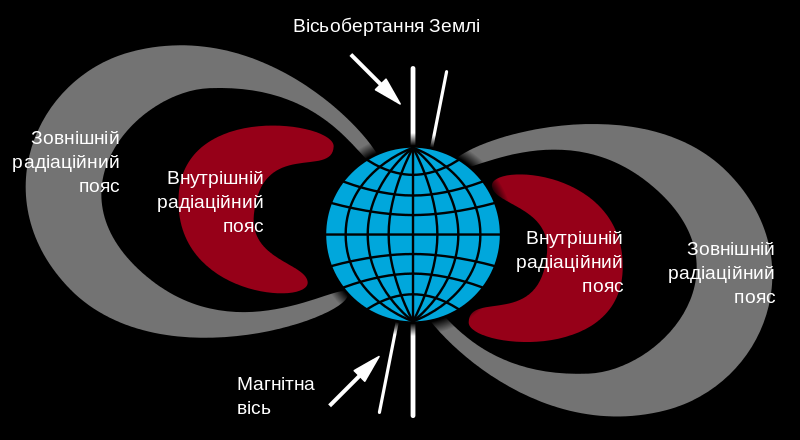
\includegraphics[width=\linewidth]{Allen_radiation_belt}
       \end{subfigure}
       %---------------------------------------------------------
       \begin{subfigure}[t]{0.4\linewidth}\centering
           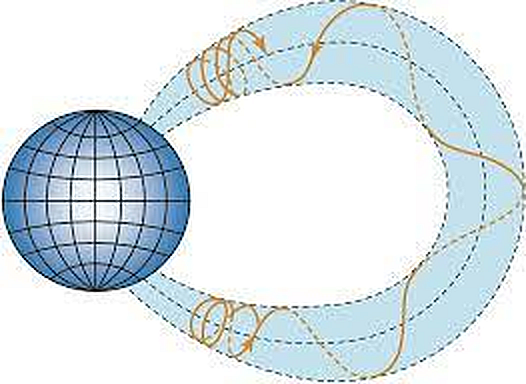
\includegraphics[width=\linewidth]{Belt_trap}
       \end{subfigure}
       %---------------------------------------------------------
       \end{figure}
       %=========================================================
       \begin{block}{}\justifying\scriptsize
           Внутрішній радіаційний пояс на висоті бл. $40\ 00$~км, що складається переважно з протонів з енергією в десятки та сотні МеВ, зовнішній ---  на висоті бл. $17\ 000$~км, що складається переважно з електронів з енергією в десятки кеВ.
       \end{block}
       \begin{exampleblock}{}\justifying\scriptsize
           Одне коливання вздовж силової лінії протон з енергією $100$~Мев здійснює за час близько $0.3$~с. Час перебування такого протона в геомагнітній пастці може сягати $100$~років, за цей час він може зробити до $10^{10}$ коливань.
       \end{exampleblock}
\end{frame}
% ===========================================================================




% ============================== Слайд ## ===================================
\begin{frame}{Багатодзеркальне утримання}{}
       \begin{center}
           \begin{tikzpicture}
        \path[name path=A, domain=-3/2*pi:3/2*pi, samples=250] plot({\x}, {0.5+0.25*cos(2*\x r)});
        \path[name path=B, domain=-3/2*pi:3/2*pi, samples=250] plot({\x}, {-0.5-0.25*cos(2*\x r)});
        \tikzfillbetween[of=A and B]{red, opacity=0.1};
\end{tikzpicture}
       \end{center}
       \begin{block}{}\justifying
          В ланцюжку пасток, частинка, що вилітає з області утримання, може захопитися іншою пасткою, погойдатись від дзеркала до дзеркала і знову розсіятися в довільному напрямку. Час, який частинці знадобиться на шлях від початку пастки до її кінця, квадратично зростає зі зростанням довжини (випадкові блукання).
       \end{block}
\end{frame}
% ===========================================================================

% ============================== Слайд ## ===================================
\begin{frame}{Задачі}{}
\begin{onlyenv}<1>
       \begin{exampleblock}{Задача 1}\justifying% Чен 2.10
       % https://www.wolframalpha.com/input?i=sin%28pi%2F4%29*3e10%2F%284.8e-10+*+700%29*sqrt%282*3.34e-24*3.204e-8%29
           Ядро атома дейтерію з енергією $20$~кеВ рухається під пітч-кутом $\theta = 45^\circ$ у центральній площині пастки з $B = 700$~Гс. Обчисліть ларморівський радіус частинки.
       \end{exampleblock}
\end{onlyenv}
\begin{onlyenv}<2>
       \begin{exampleblock}{Задача 2}\justifying% Чен 2.12
           Протон із космічних променів захоплений у пастці між двома
           рухомими магнітними дзеркалами з дзеркальним відношенням $5$. В  початковий момент у центральній площині енергія частинки $E = 1$~кеВ, причому $v_\perp= v_\parallel$. Кожна з пробок рухається до центру системи зі швидкістю $v = 10$~км/с. Знайдіть енергію, до якої буде прискорено протон, перш ніж він покине систему. Скільки часу знадобиться на те, щоб набрати цю енергію?
           Початкова відстань між дзеркалами $L = 10^{10}$~км.

           \smallskip

           \emph{Вказівка}: В якості моделі, дзеркала можна вважати плоскими поршнями, від стінок яких відбувається пружне відбиття частинки.


           \bigskip

           {\scriptsize Магнітне дзеркало вперше було запропоновано Енріко Фермі для пояснення механізму прискорення космічних променів. Він помітив, що протони, які осцилюють між двома магнітними дзеркалами, що зближуються з великою швидкістю, можуть під час кожного прольоту між ними збільшувати свою енергію.}

       \end{exampleblock}
\end{onlyenv}
\end{frame}
% ===========================================================================

\end{document}

